\section{Komunia Święta \textit{bardziej uroczysta}}

\subsection{Komunia Święta dwójkami – bez obrusu komunijnego}

\begin{itemize}
	\item Ministranci biorący udział w lucenarium wchodzą dwójkami do
	      prezbiterium, tworząc w ten sposób naturalną „kolejkę”. Przed nimi do
	      kolejki wchodzą \aa\aa~, trzymając w rękach patenę. Za nimi miejsce
	      zajmuje \cc~ razem z \tt~ lub innym ministrantem.
	\item Na znak \cc cała procesja komunijna najpierw przyklęka, a potem klęka
	      na dwa kolana. \aa\aa~ wchodzą na najwyższy stopień ołtarza i
	      przyjmują Komunię Świętą jako pierwsi.
	\item \aa\aa~ po przyjęciu Komunii Świętej na najwyższym stopniu ołtarza i
	      przyklęknięciu zajmują miejsce przy celebransie z pateną i świeczką
	      sanctusową.
	\item Każda para tuż przed przyjęciem Komunii Świętej przyklęka na podłodze,
	      razem z parą poprzedzającą, która już Komunię przyjęła.
	\item Każda para po przyjęciu Komunii Świętej przyklęka, po czym odchodzi na
	      stronę Ewangelii, w kierunku chóru.
\end{itemize}

\subsection{Śpiewana bardziej uroczysta – z obrusem komunijnym}

\begin{itemize}
	\item Podczas śpiewu \textit{Agnus Dei} \aa1 bierze z kredencji obrus
	      komunijny, razem z \aa2 klękają pośrodku, wchodzą na najwyższy stopień
	      ołtarza i klęcząc przodem do siebie trzymają rozłożony obrus (Rys.
	      \ref{fig:komunia_1}).

	      \begin{figure}[h]
		      \centering
		      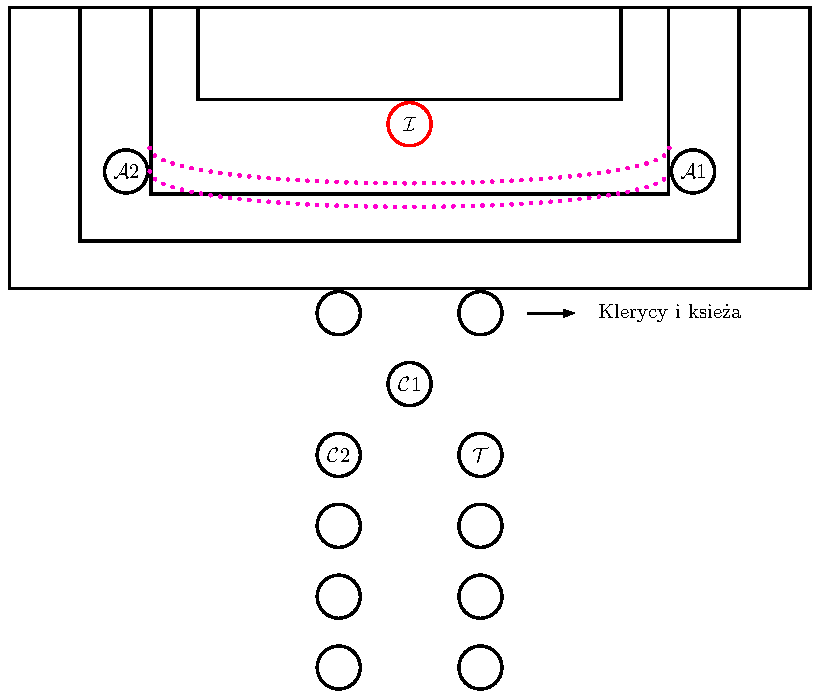
\includegraphics[width=0.5\linewidth]{komunia_1}
		      \caption{Procesja do Komunii Św.}
		      \label{fig:komunia_1}
	      \end{figure}

	\item Ministranci biorący udział w lucenarium wchodzą dwójkami do
	      prezbiterium, tworząc w ten sposób naturalną „kolejkę” do Komunii św.
	      Przed nimi do kolejki wchodzą księża, klerycy i \cc~, za nimi reszta
	      ministrantów z chóru. \cc1 – zależnie od ilości duchownych i
	      ministrantów może staje do komunii sam lub w parze.
	\item \cc~ podaje patenę pierwszemu duchownemu przyjmującemu Komunię św.,
	      albo jeśli nie ma duchownych trzyma ją sam. Po przyjęciu Komunii Św.
	      zajmuje miejsce przy \ii, gdzie asystuje z pateną.
	\item \cc2 lub \tt~ po przyjęciu Komunii św. zajmuje miejsce przy \ii~ ze
	      świeczką sanctusową (Rys. \ref{fig:komunia_2}).

	      \begin{figure}[h]
		      \centering
		      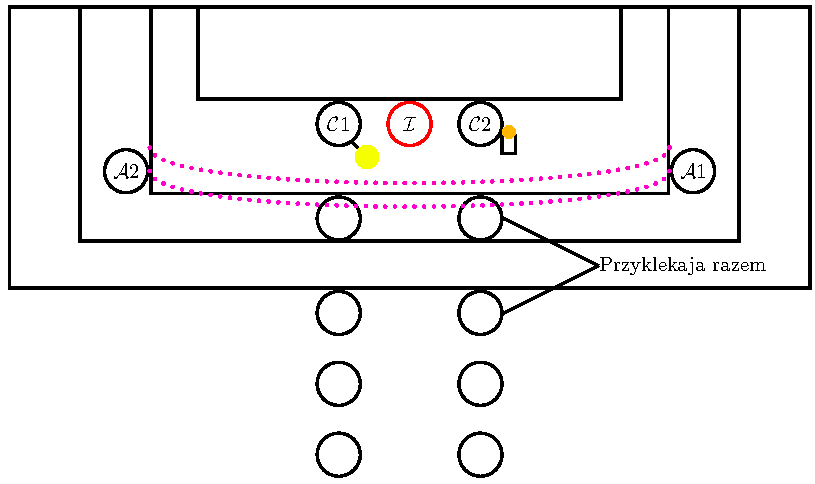
\includegraphics[width=0.5\linewidth]{komunia_2}
		      \caption{W trakcie udzielania Komunii Św. ministrantom}
		      \label{fig:komunia_2}
	      \end{figure}

	\item \aa\aa~ trzymający obrus przyjmują Komunię św. razem z \cc1.
	\item Każda dwójka przystępująca do Komunii św. przyklęka jednocześnie z
	      poprzedzającą parą, wchodzi na stopnie i klęka na dwa kolana. Po
	      przyjęciu komunii znów przyklęka jednocześnie z parą stojącą za nimi.
	      Ze stopni ołtarza schodzimy w lewo – do chóru.
	\item Po przyjęciu Komunii Św. przez ministrantów \aa\aa~ wstają i
	      przechodzą do miejsca udzielania komunii wiernym. Z pateną i świeczką
	      sanctusową asystują \cc\cc~ (Rys. \ref{fig:komunia_3}).

	      \begin{figure}[h]
		      \centering
		      \includegraphics[width=0.5\linewidth]{komunia_3}
		      \caption{W trakcie udzielania Komunii Św. ludowi}
		      \label{fig:komunia_3}
	      \end{figure}

\end{itemize}

\clearpage

\subsection{Msza solenna -- bez obrusu komunijnego}

\begin{itemize}
	\item Podczas śpiewu \textit{Agnus Dei} przekazywany jest znak pokoju – \ss~
	      przekazuje go duchownym w chórze i \cc\cc.
	\item Ministranci biorący udział w lucenarium wchodzą dwójkami do
	      prezbiterium, tworząc w ten sposób naturalną „kolejkę” do Komunii św.
	      Zostawiają przed sobą miejsce dla duchownych, mających przyjąć
	      Komunię. Za nimi ustawia się reszta ministrantów (Rys.
	      \ref{fig:komunia_1_uro_bez})
	\item Jeśli \dd~ lub inny kapłan rozdaje Komunię św., \cc~ asystuje ze
	      świeczką \ii, a \aa\aa~ z pateną i świeczką asystują \dd~ (Rys.
	      \ref{fig:komunia_3_uro_diak_bez}).

	      \begin{figure}[ht]
		      \centering
		      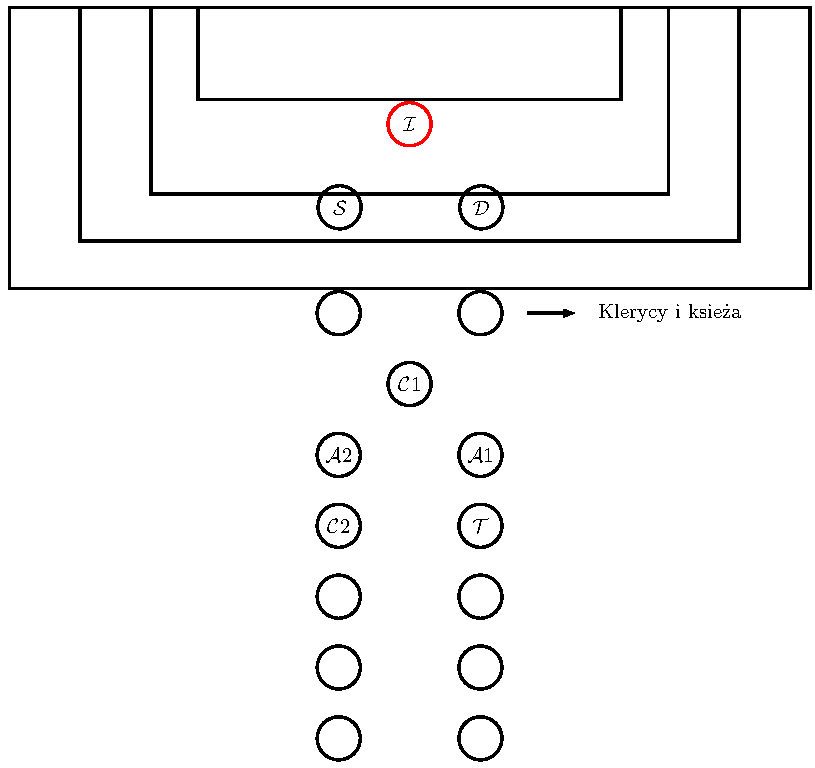
\includegraphics[width=0.5\linewidth]{komunia_1_uro_bez}
		      \caption{W trakcie udzielania Komunii Św. ludowi (diakon rozdaje)}
		      \label{fig:komunia_1_uro_bez}
	      \end{figure}

	      \begin{figure}[ht]
		      \centering
		      \includegraphics[width=0.5\linewidth]{komunia_3_uro_diak_bez}
		      \caption{W trakcie udzielania Komunii Św. ludowi (diakon rozdaje)}
		      \label{fig:komunia_3_uro_diak_bez}
	      \end{figure}
\end{itemize}

\subsection{Msza solenna -- z obrusem komunijnym}

\begin{itemize}
	\item Po ewentualnym. odebraniu znaku pokoju \aa1 bierze z kredencji obrus
	      komunijny, razem z \aa2 klękają pośrodku, wchodzą na najwyższy stopień
	      ołtarza i klęcząc przodem do siebie trzymają rozłożony obrus.
	\item Porządek Komunii Św. (patrz obrazki przy mszy śpiewanej z obrusem)
	      \begin{itemize}
		      \item \dd~ i \ss~
		      \item kapłani, klerycy
		      \item \aa\aa~ trzymający obrus i \cc1
		      \item \cc2 i \tt~
		      \item reszta ministrantów.
	      \end{itemize}
	\item Jeśli \dd~ nie rozdaje komunii, razem z \ss~ asystują \ii. Podąża za
	      nimi \cc1 ze świeczką sanctusową (Rys. \ref{fig:komunia_3_uro}).

	      \begin{figure}[h]
		      \centering
		      \includegraphics[width=0.5\linewidth]{komunia_3_uro}
		      \caption{W trakcie udzielania Komunii Św. ludowi (\dd~ nie rozdaje)}
		      \label{fig:komunia_3_uro}
	      \end{figure}

	\item Jeśli \dd~ lub inny kapłan rozdaje komunię przy obrusie (Rys.
	      \ref{fig:komunia_3_uro_1}):

	      \begin{itemize}
		      \item \ii~ asystuje \ss~ z pateną
		      \item \dd~ asystuje \cc2 z pateną
		      \item dwóch wyznaczonych ministrantów z chóru po przyjęciu Komunii
		            zapala świeczki i przy udzielaniu komunii wiernym, klęczą ze
		            świeczkami po dwóch stronach obrusa.
	      \end{itemize}

	      \begin{figure}[ht]
		      \centering
		      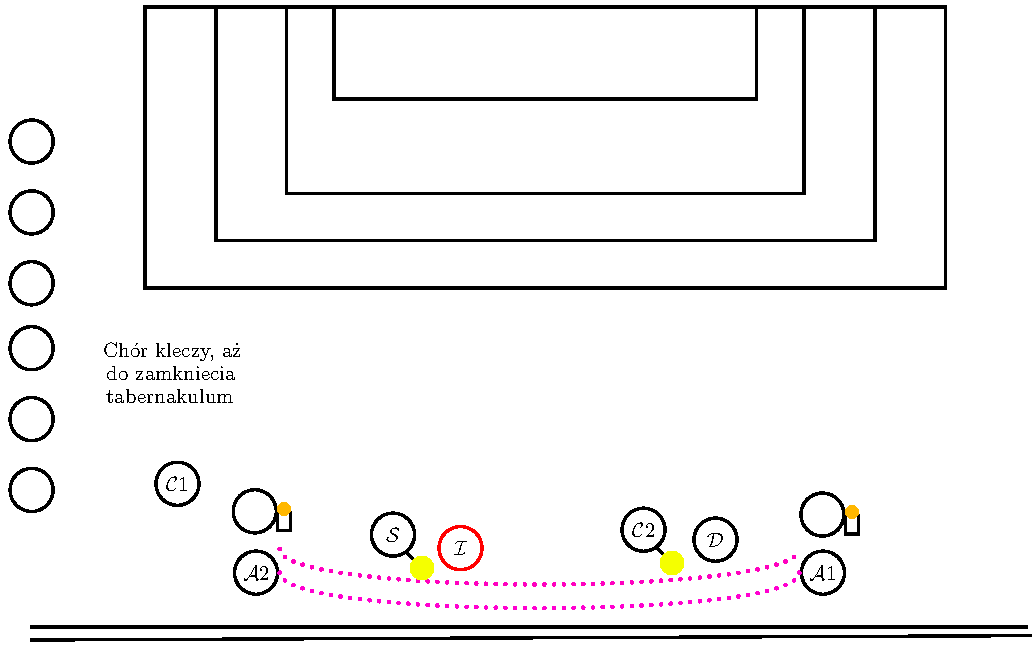
\includegraphics[width=0.5\linewidth]{komunia_3_uro_diak}
		      \caption{W trakcie udzielania Komunii Św. ludowi (\dd~ rozdaje)}
		      \label{fig:komunia_3_uro_1}
	      \end{figure}

\end{itemize}

\clearpage
